\documentclass[tikz,border=1pt]{standalone}
\usepackage{pgfplots}
\pgfplotsset{compat=1.18}
\usepgfplotslibrary{groupplots}
\begin{document}
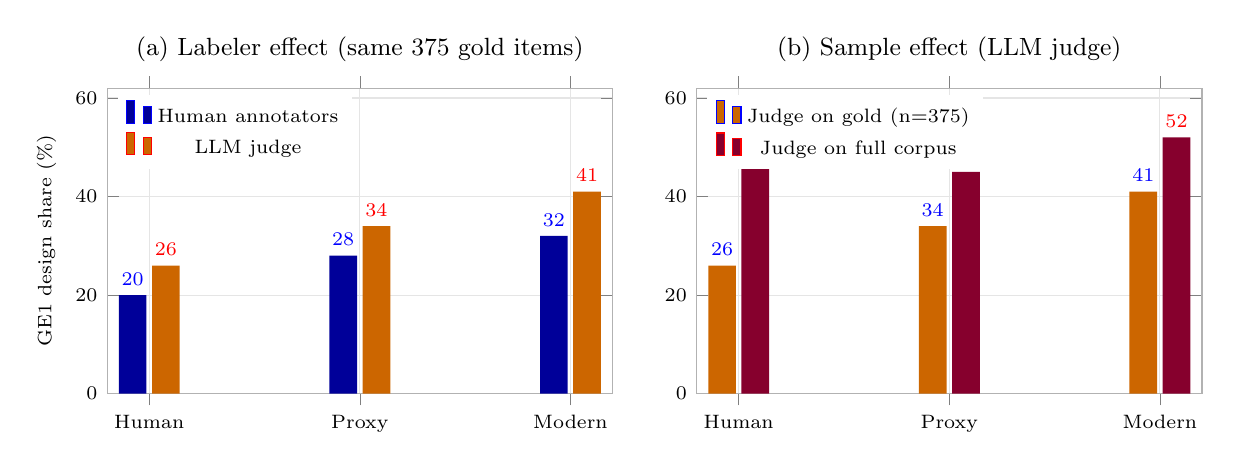
\begin{tikzpicture}
\begin{groupplot}[
  group style={group size=2 by 1,horizontal sep=0.42in},
  width=3.15in,
  height=2.15in,
  ybar,
  ymin=0,
  ymax=62,
  ylabel style={font=\scriptsize},
  yticklabel style={font=\scriptsize},
  xtick={0,1,2},
  xticklabels={Human,Proxy,Modern},
  x tick label style={font=\scriptsize},
  tick label style={font=\scriptsize},
  title style={font=\small},
  legend style={draw=none,font=\scriptsize,at={(0.02,0.98)},anchor=north west},
  grid=major,
  grid style={draw=gray!20},
  axis line style={gray!60},
  nodes near coords,
  every node near coord/.append style={font=\scriptsize,anchor=south},
]
\nextgroupplot[
  title={(a) Labeler effect (same 375 gold items)},
  ylabel={GE1 design share (\%)},
]
\addplot+[fill=blue!60!black,draw=none] coordinates {(0,20) (1,28) (2,32)};
\addlegendentry{Human annotators}
\addplot+[fill=orange!80!black,draw=none] coordinates {(0,26) (1,34) (2,41)};
\addlegendentry{LLM judge}

\nextgroupplot[
  title={(b) Sample effect (LLM judge)},
]
\addplot+[fill=orange!80!black,draw=none] coordinates {(0,26) (1,34) (2,41)};
\addlegendentry{Judge on gold (n=375)}
\addplot+[fill=purple!70!black,draw=none] coordinates {(0,51) (1,45) (2,52)};
\addlegendentry{Judge on full corpus}
\end{groupplot}
\end{tikzpicture}
\end{document}
